\section{Resultados de algoritmos de clasificación}

Este documento explica los avances realizados de la semana 8 a la 10 el cual corresponde al perido 22 de septiembre $-$ 12 de octubre( ver Figura \ref{fig:cronograma}) del año 2019. las actividades realizadas son:

\begin{enumerate}
	\item Recolección de noticias para incrementar el corpus de 500 a 700 noticias por sección
	\item Aplicación de filtro de número de palabras mínimas	
	\item Entrenamiento de los algoritmos \textbf{naive bayes}, \textbf{random forest}, \textbf{maquina de soporte vectorial},\textbf{regresión logística}
	\item Reporte de resultados del entrenamiento
	\item Diseño de la página web
\end{enumerate} 

\begin{figure}[h]
\centering
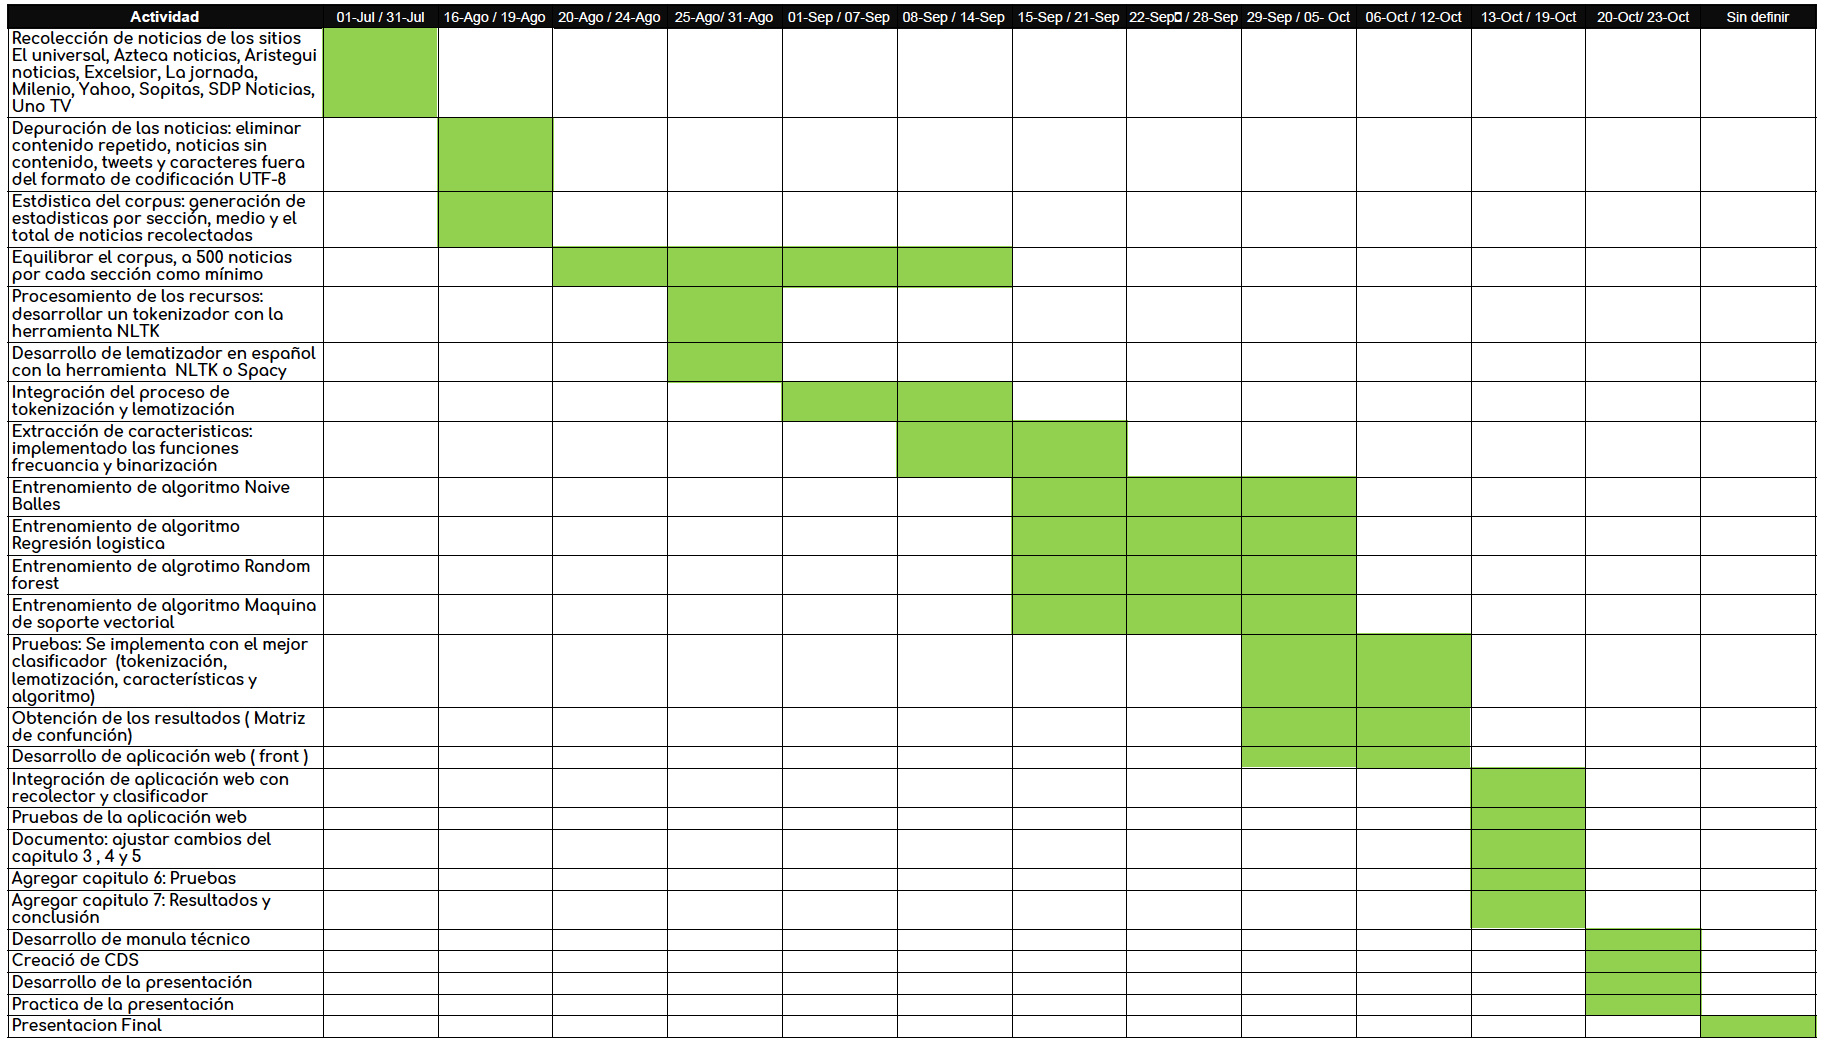
\includegraphics[scale=0.4]{imagenes/Cronograma.png}
\caption{Crononograma correspondiente al trabajo terminal 2}
\label{fig:cronograma}
\end{figure}

%--------------------------------------------------------------------------------------------------%
\section{Recolección de noticias para incrementar el corpus}

Como meta del número de noticias para formar el corpus se propuso 500 noticias por cada sección ( las cuales son \textbf{ciencia y tecnología}, \textbf{deportes}, \textbf{política}, \textbf{cultura} y \textbf{economía}) sin embargo con la motivación de alcanzar mejores resultados en el entrenamiento de los algoritmos antes mencionados, se incremento el número de artículos a 700, es decir 3500 noticias en total.\\

Para este procedimiento se recolectaban noticias cada 3 días de los sitios web:

\begin{itemize}
	  \item \textbf{El Universal}: https://www.eluniversal.com.mx/
      \item \textbf{La Jornada}: https://www.jornada.com.mx/
	  \item \textbf{Aristegui Noticias}: https://aristeguinoticias.com/
	  \item \textbf{Sopitas}: https://www.sopitas.com/
      \item \textbf{TV Azteca}: https://www.aztecanoticias.com.mx/
      \item \textbf{Televisa}: https://noticieros.televisa.com/
      \item \textbf{Once Noticias}: https://www.oncenoticias.tv/
      \item \textbf{El economista}: https://www.eleconomista.com.mx/
\end{itemize}

Se implementaron las arañas (\textit{crawlers}) desarrolladas en el trabajo terminal 1. Además se espesializaron algunos algoritmos para obtener mas noticias de las previamente programas.\\

El resultado de las noticias recoleactadas se muestra en la Figura 

\begin{figure}[h]
\centering
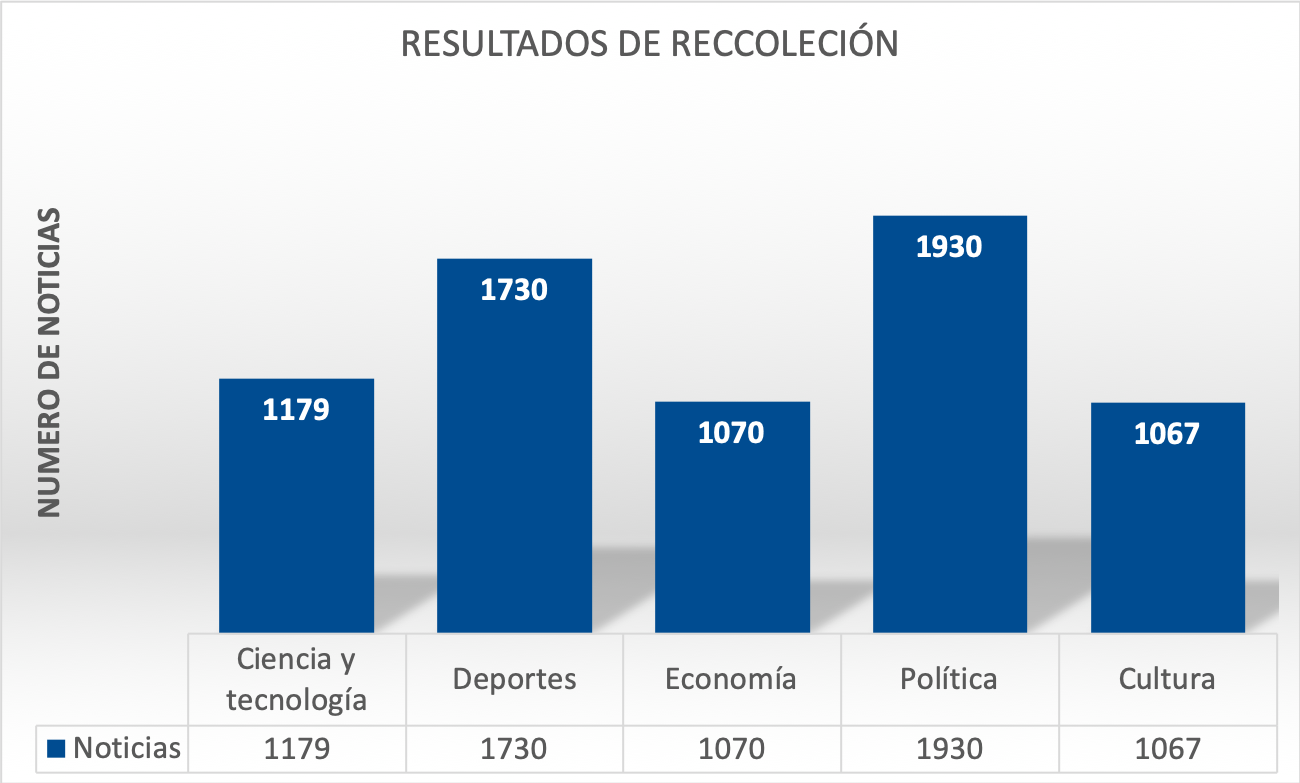
\includegraphics[scale=0.35]{imagenes/Resultados/Recoleccion.png}
\caption{Gráfica de recolección de noticias}
\label{fig:recoleccion}
\end{figure}

%--------------------------------------------------------------------------------------------------%
\section{Aplicación de filtro de número de palabras mínimas}

Una vez obtenidas las noticias se limpiaron y se filtraron por el número de palabras mínimas el cual es 180. El número de artículos  obtenidos se muestra en la siguiente figura.

\begin{figure}[h]
\centering
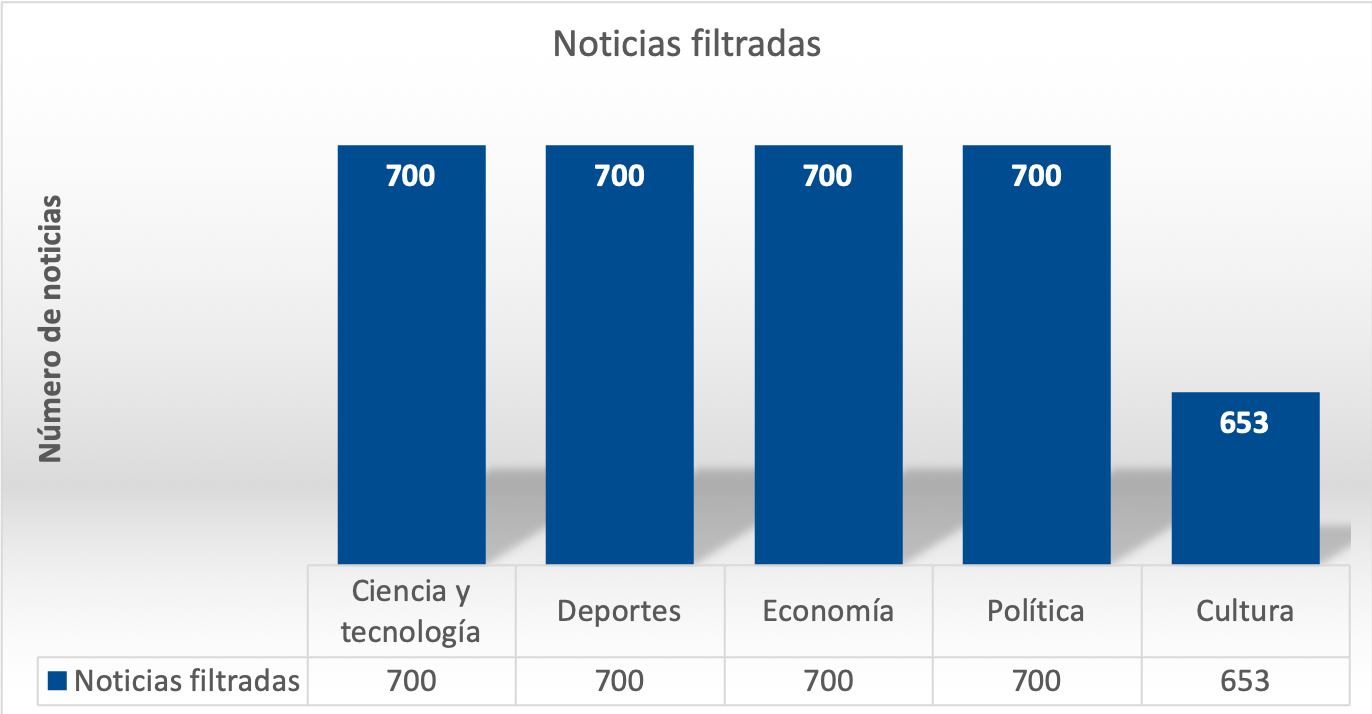
\includegraphics[scale=0.35]{imagenes/Resultados/Filtrado.png}
\caption{Gráfica de noticias obtenidas con mas de 180 palabras}
\label{fig:filtro}
\end{figure}



\section{Reporte de resultados del entrenamiento}


\begin{figure}[h]
\centering
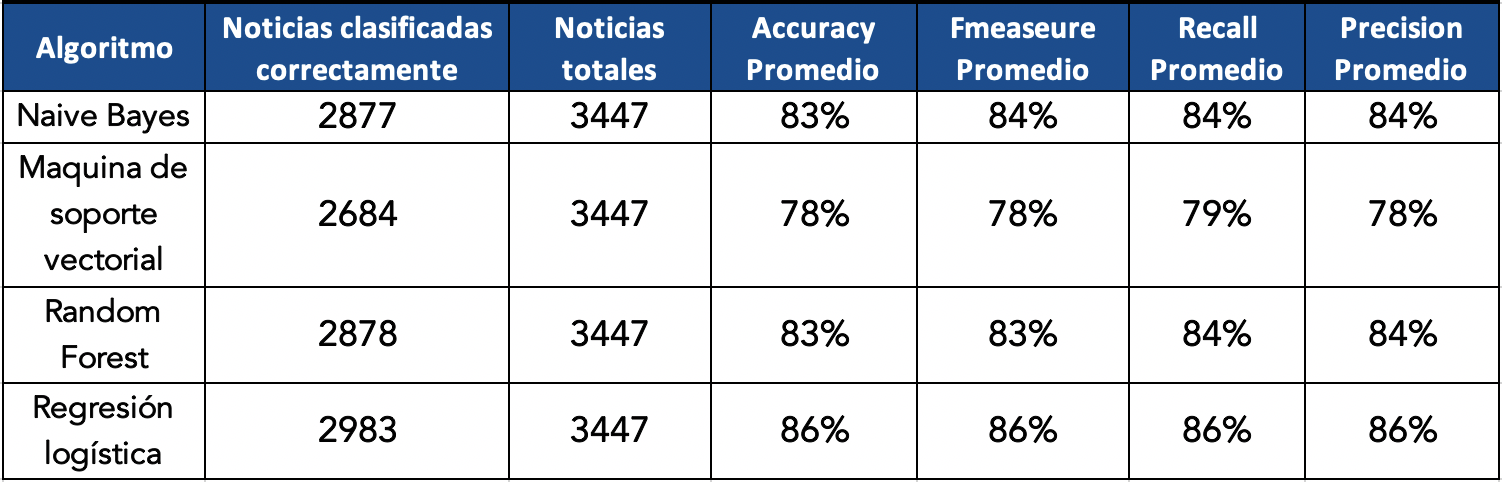
\includegraphics[scale=0.35]{imagenes/Resultados/MatrizFrecuencia.png}
\caption{Resultados de entrenamiento modo Frecuencia}
\label{fig:matrizfrecuencia}
\end{figure}

\begin{figure}[h]
\centering
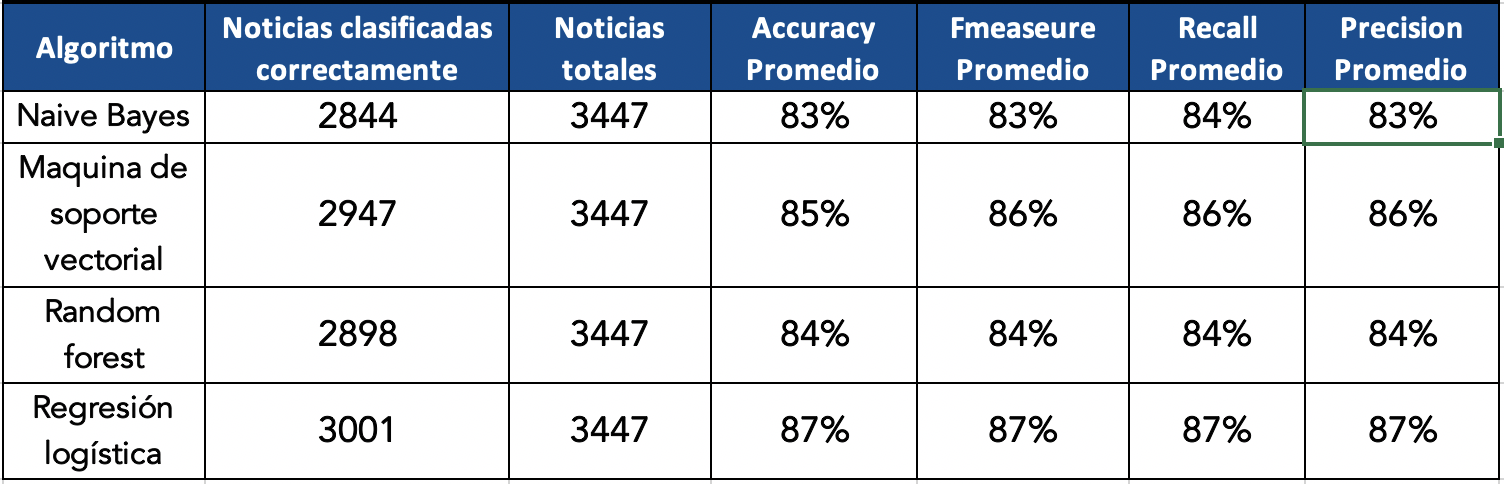
\includegraphics[scale=0.35]{imagenes/Resultados/MatrizBinario.png}
\caption{Resultados de entrenamiento en modo binario}
\label{fig:matrizbinario}
\end{figure}